\PassOptionsToPackage{dvipsnames,table}{xcolor}
\documentclass[11pt,a4paper]{article}

\usepackage{DS}

\begin{document}
\newcommand{\ModeExercice}{
% Traduction des noms pour le package exercise
\renewcommand{\ExerciseName}{Exercice}
\renewcommand{\thesubQuestion}{\theQuestion.\alph{subQuestion}}
\renewcommand{\AnswerName}{Réponses à l'exercise }
}
\newcommand{\Fiche}[2]{\lhead{\textbf{{\sc #1}}}
\rhead{Niveau: \textbf{#2}}
\cfoot{}}
\definecolor{cfond}{gray}{0.4}
\renewcommand{\thealgocf}{}

\newcommand{\ModeActivite}{
% Traduction des noms pour le package exercise
\renewcommand{\ExerciseName}{Activité}
}
% Réglages de la mise en forme des exercices 
\renewcommand{\ExerciseHeaderTitle}{\ExerciseTitle}
\renewcommand{\ExerciseHeaderOrigin}{\ExerciseOrigin}
% Un : sépare le numéro de l'exerice de son titre ... si le titre existe. On utilise Origine pour placer les pictogrammes en fin de ligne
\renewcommand{\ExerciseHeader}{\ding{113} \textbf{\sffamily{\ExerciseName \ \ExerciseHeaderNB}} \ifthenelse{\equal{\ExerciseTitle}{\empty}}{}{:} \textit{\ExerciseHeaderTitle} \hfill \ExerciseHeaderOrigin}
\renewcommand{\ExePartHeader}{\quad {\footnotesize \ding{110}} \textbf{Partie \textbf{\ExePartHeaderNB}} : \ExePartName}


% Mode Concours
\newcommand{\ModeConcours}{
   \newcounter{qconcours}
   \setcounter{qconcours}{1}
   \renewcommand{\ExerciseName}{Exercice}
   \renewcommand{\ExerciseHeaderTitle}{\ExerciseTitle}
\renewcommand{\ExerciseHeaderOrigin}{\ExerciseOrigin}
\renewcommand{\ExerciseHeader}{\ding{113} \textbf{\sffamily{\ExerciseName \ \ExerciseHeaderNB}} \ifthenelse{\equal{\ExerciseTitle}{\empty}}{}{:} \textit{\ExerciseHeaderTitle} \hfill \ExerciseHeaderOrigin}
\renewcommand{\QuestionNB}{\textbf{Q\arabic{qconcours}--}\ \addtocounter{qconcours}{1}}}

\newcommand{\noeud}[1]{\Tr{\fbox{\tt #1}}}
\newcommand{\FPATH}{/home/fenarius/Travail/Cours/cpge-info/docs/mp2i/}
\newcommand{\spath}[2]{\FPATH Evaluations/#1/#1#2}
\definecolor{codebg}{gray}{0.90}
\newcommand{\inputpartOCaml}[5]{\begin{mdframed}[backgroundcolor=codebg] \inputminted[breaklines=true,fontsize=#3,linenos=true,highlightcolor=fluo,tabsize=2,highlightlines={#2},firstline=#4,lastline=#5,firstnumber=1]{OCaml}{#1} \end{mdframed}}
\newcommand{\inputpartPython}[5]{\begin{mdframed}[backgroundcolor=codebg] \inputminted[breaklines=true,fontsize=#3,linenos=true,highlightcolor=fluo,tabsize=2,highlightlines={#2},firstline=#4,lastline=#5,firstnumber=1]{python}{#1} \end{mdframed}}
\newcommand{\inputpartC}[5]{\begin{mdframed}[backgroundcolor=codebg] \inputminted[breaklines=true,fontsize=#3,linenos=true,highlightcolor=fluo,tabsize=2,highlightlines={#2},firstline=#4,lastline=#5,firstnumber=1]{c}{#1} \end{mdframed}}
\newcommand{\inputC}[2]{\begin{mdframed}[backgroundcolor=codebg] \inputminted[breaklines=true,fontsize=#2,linenos=true,highlightcolor=fluo,tabsize=2]{c}{#1} \end{mdframed}}
\newminted[langageC]{c}{linenos=true,escapeinside=``,highlightcolor=fluo,tabsize=2}
\newminted[python]{python}{linenos=true,escapeinside=``,highlightcolor=fluo,tabsize=4}
\BeforeBeginEnvironment{minted}{\begin{mdframed}[backgroundcolor=codebg,skipabove=0cm]}
   \AfterEndEnvironment{minted}{\end{mdframed}}

% Font light medium et bold pour tt :
\newcommand{\ttl}[1]{\ttfamily \fontseries{l}\selectfont #1}
\newcommand{\ttm}[1]{\ttfamily \fontseries{m}\selectfont #1}
\newcommand{\ttb}[1]{\ttfamily \fontseries{b}\selectfont #1}

%QCM de NSI \QNSI{Question}{R1}{R2}{R3}{R4}
\newcommand{\QNSI}[5]{
#1
\begin{enumerate}[label=\alph{enumi})]
\item #2
\item #3
\item #4
\item #5
\end{enumerate}
}



\definecolor{grispale}{gray}{0.95}
\newcommand{\htmlmode}{\lstset{language=html,numbers=left, tabsize=2, frame=single, breaklines=true, keywordstyle=\ttfamily, basicstyle=\small,
   numberstyle=\tiny\ttfamily, framexleftmargin=0mm, backgroundcolor=\color{grispale}, xleftmargin=12mm,showstringspaces=false}}
\newcommand{\pythonmode}{\lstset{language=python,numbers=left, tabsize=4, frame=single, breaklines=true, keywordstyle=\ttfamily, basicstyle=\small,
   numberstyle=\tiny\ttfamily, framexleftmargin=0mm, backgroundcolor=\color{grispale}, xleftmargin=12mm, showstringspaces=false}}
\newcommand{\bashmode}{\lstset{language=bash,numbers=left, tabsize=2, frame=single, breaklines=true, basicstyle=\ttfamily,
   numberstyle=\tiny\ttfamily, framexleftmargin=0mm, backgroundcolor=\color{grispale}, xleftmargin=12mm, showstringspaces=false}}
\newcommand{\exomode}{\lstset{language=python,numbers=left, tabsize=2, frame=single, breaklines=true, basicstyle=\ttfamily,
   numberstyle=\tiny\ttfamily, framexleftmargin=13mm, xleftmargin=12mm, basicstyle=\small, showstringspaces=false}}
   
   
  \lstset{%
        inputencoding=utf8,
        extendedchars=true,
        literate=%
        {é}{{\'{e}}}1
        {è}{{\`{e}}}1
        {ê}{{\^{e}}}1
        {ë}{{\¨{e}}}1
        {É}{{\'{E}}}1
        {Ê}{{\^{E}}}1
        {û}{{\^{u}}}1
        {ù}{{\`{u}}}1
        {ú}{{\'{u}}}1
        {â}{{\^{a}}}1
        {à}{{\`{a}}}1
        {á}{{\'{a}}}1
        {ã}{{\~{a}}}1
        {Á}{{\'{A}}}1
        {Â}{{\^{A}}}1
        {Ã}{{\~{A}}}1
        {ç}{{\c{c}}}1
        {Ç}{{\c{C}}}1
        {õ}{{\~{o}}}1
        {ó}{{\'{o}}}1
        {ô}{{\^{o}}}1
        {Õ}{{\~{O}}}1
        {Ó}{{\'{O}}}1
        {Ô}{{\^{O}}}1
        {î}{{\^{i}}}1
        {Î}{{\^{I}}}1
        {í}{{\'{i}}}1
        {Í}{{\~{Í}}}1
}

%tei pour placer les images
%tei{nom de l’image}{échelle de l’image}{sens}{texte a positionner}
%sens ="1" (droite) ou "2" (gauche)
\newlength{\ltxt}
\newcommand{\tei}[4]{
\setlength{\ltxt}{\linewidth}
\setbox0=\hbox{\includegraphics[scale=#2]{#1}}
\addtolength{\ltxt}{-\wd0}
\addtolength{\ltxt}{-10pt}
\ifthenelse{\equal{#3}{1}}{
\begin{minipage}{\wd0}
\includegraphics[scale=#2]{#1}
\end{minipage}
\hfill
\begin{minipage}{\ltxt}
#4
\end{minipage}
}{
\begin{minipage}{\ltxt}
#4
\end{minipage}
\hfill
\begin{minipage}{\wd0}
\includegraphics[scale=#2]{#1}
\end{minipage}
}
}

%Juxtaposition d'une image pspciture et de texte 
%#1: = code pstricks de l'image
%#2: largeur de l'image
%#3: hauteur de l'image
%#4: Texte à écrire
\newcommand{\ptp}[4]{
\setlength{\ltxt}{\linewidth}
\addtolength{\ltxt}{-#2 cm}
\addtolength{\ltxt}{-0.1 cm}
\begin{minipage}[b][#3 cm][t]{\ltxt}
#4
\end{minipage}\hfill
\begin{minipage}[b][#3 cm][c]{#2 cm}
#1
\end{minipage}\par
}



%Macros pour les graphiques
\psset{linewidth=0.5\pslinewidth,PointSymbol=x}
\setlength{\fboxrule}{0.5pt}
\newcounter{tempangle}

%Marque la longueur du segment d'extrémité  #1 et  #2 avec la valeur #3, #4 est la distance par rapport au segment (en %age de la valeur de celui ci) et #5 l'orientation du marquage : +90 ou -90
\newcommand{\afflong}[5]{
\pstRotation[RotAngle=#4,PointSymbol=none,PointName=none]{#1}{#2}[X] 
\pstHomO[PointSymbol=none,PointName=none,HomCoef=#5]{#1}{X}[Y]
\pstTranslation[PointSymbol=none,PointName=none]{#1}{#2}{Y}[Z]
 \ncline{|<->|,linewidth=0.25\pslinewidth}{Y}{Z} \ncput*[nrot=:U]{\footnotesize{#3}}
}
\newcommand{\afflongb}[3]{
\ncline{|<->|,linewidth=0}{#1}{#2} \naput*[nrot=:U]{\footnotesize{#3}}
}

%Construis le point #4 situé à #2 cm du point #1 avant un angle #3 par rapport à l'horizontale. #5 = liste de paramètre
\newcommand{\lsegment}[5]{\pstGeonode[PointSymbol=none,PointName=none](0,0){O'}(#2,0){I'} \pstTranslation[PointSymbol=none,PointName=none]{O'}{I'}{#1}[J'] \pstRotation[RotAngle=#3,PointSymbol=x,#5]{#1}{J'}[#4]}
\newcommand{\tsegment}[5]{\pstGeonode[PointSymbol=none,PointName=none](0,0){O'}(#2,0){I'} \pstTranslation[PointSymbol=none,PointName=none]{O'}{I'}{#1}[J'] \pstRotation[RotAngle=#3,PointSymbol=x,#5]{#1}{J'}[#4] \pstLineAB{#4}{#1}}

%Construis le point #4 situé à #3 cm du point #1 et faisant un angle de  90° avec la droite (#1,#2) #5 = liste de paramètre
\newcommand{\psegment}[5]{
\pstGeonode[PointSymbol=none,PointName=none](0,0){O'}(#3,0){I'}
 \pstTranslation[PointSymbol=none,PointName=none]{O'}{I'}{#1}[J']
 \pstInterLC[PointSymbol=none,PointName=none]{#1}{#2}{#1}{J'}{M1}{M2} \pstRotation[RotAngle=-90,PointSymbol=x,#5]{#1}{M1}[#4]
  }
  
%Construis le point #4 situé à #3 cm du point #1 et faisant un angle de  #5° avec la droite (#1,#2) #6 = liste de paramètre
\newcommand{\mlogo}[6]{
\pstGeonode[PointSymbol=none,PointName=none](0,0){O'}(#3,0){I'}
 \pstTranslation[PointSymbol=none,PointName=none]{O'}{I'}{#1}[J']
 \pstInterLC[PointSymbol=none,PointName=none]{#1}{#2}{#1}{J'}{M1}{M2} \pstRotation[RotAngle=#5,PointSymbol=x,#6]{#1}{M2}[#4]
  }

% Construis un triangle avec #1=liste des 3 sommets séparés par des virgules, #2=liste des 3 longueurs séparés par des virgules, #3 et #4 : paramètre d'affichage des 2e et 3 points et #5 : inclinaison par rapport à l'horizontale
%autre macro identique mais sans tracer les segments joignant les sommets
\noexpandarg
\newcommand{\Triangleccc}[5]{
\StrBefore{#1}{,}[\pointA]
\StrBetween[1,2]{#1}{,}{,}[\pointB]
\StrBehind[2]{#1}{,}[\pointC]
\StrBefore{#2}{,}[\coteA]
\StrBetween[1,2]{#2}{,}{,}[\coteB]
\StrBehind[2]{#2}{,}[\coteC]
\tsegment{\pointA}{\coteA}{#5}{\pointB}{#3} 
\lsegment{\pointA}{\coteB}{0}{Z1}{PointSymbol=none, PointName=none}
\lsegment{\pointB}{\coteC}{0}{Z2}{PointSymbol=none, PointName=none}
\pstInterCC{\pointA}{Z1}{\pointB}{Z2}{\pointC}{Z3} 
\pstLineAB{\pointA}{\pointC} \pstLineAB{\pointB}{\pointC}
\pstSymO[PointName=\pointC,#4]{C}{C}[C]
}
\noexpandarg
\newcommand{\TrianglecccP}[5]{
\StrBefore{#1}{,}[\pointA]
\StrBetween[1,2]{#1}{,}{,}[\pointB]
\StrBehind[2]{#1}{,}[\pointC]
\StrBefore{#2}{,}[\coteA]
\StrBetween[1,2]{#2}{,}{,}[\coteB]
\StrBehind[2]{#2}{,}[\coteC]
\tsegment{\pointA}{\coteA}{#5}{\pointB}{#3} 
\lsegment{\pointA}{\coteB}{0}{Z1}{PointSymbol=none, PointName=none}
\lsegment{\pointB}{\coteC}{0}{Z2}{PointSymbol=none, PointName=none}
\pstInterCC[PointNameB=none,PointSymbolB=none,#4]{\pointA}{Z1}{\pointB}{Z2}{\pointC}{Z1} 
}


% Construis un triangle avec #1=liste des 3 sommets séparés par des virgules, #2=liste formée de 2 longueurs et d'un angle séparés par des virgules, #3 et #4 : paramètre d'affichage des 2e et 3 points et #5 : inclinaison par rapport à l'horizontale
%autre macro identique mais sans tracer les segments joignant les sommets
\newcommand{\Trianglecca}[5]{
\StrBefore{#1}{,}[\pointA]
\StrBetween[1,2]{#1}{,}{,}[\pointB]
\StrBehind[2]{#1}{,}[\pointC]
\StrBefore{#2}{,}[\coteA]
\StrBetween[1,2]{#2}{,}{,}[\coteB]
\StrBehind[2]{#2}{,}[\angleA]
\tsegment{\pointA}{\coteA}{#5}{\pointB}{#3} 
\setcounter{tempangle}{#5}
\addtocounter{tempangle}{\angleA}
\tsegment{\pointA}{\coteB}{\thetempangle}{\pointC}{#4}
\pstLineAB{\pointB}{\pointC}
}
\newcommand{\TriangleccaP}[5]{
\StrBefore{#1}{,}[\pointA]
\StrBetween[1,2]{#1}{,}{,}[\pointB]
\StrBehind[2]{#1}{,}[\pointC]
\StrBefore{#2}{,}[\coteA]
\StrBetween[1,2]{#2}{,}{,}[\coteB]
\StrBehind[2]{#2}{,}[\angleA]
\lsegment{\pointA}{\coteA}{#5}{\pointB}{#3} 
\setcounter{tempangle}{#5}
\addtocounter{tempangle}{\angleA}
\lsegment{\pointA}{\coteB}{\thetempangle}{\pointC}{#4}
}

% Construis un triangle avec #1=liste des 3 sommets séparés par des virgules, #2=liste formée de 1 longueurs et de deux angle séparés par des virgules, #3 et #4 : paramètre d'affichage des 2e et 3 points et #5 : inclinaison par rapport à l'horizontale
%autre macro identique mais sans tracer les segments joignant les sommets
\newcommand{\Trianglecaa}[5]{
\StrBefore{#1}{,}[\pointA]
\StrBetween[1,2]{#1}{,}{,}[\pointB]
\StrBehind[2]{#1}{,}[\pointC]
\StrBefore{#2}{,}[\coteA]
\StrBetween[1,2]{#2}{,}{,}[\angleA]
\StrBehind[2]{#2}{,}[\angleB]
\tsegment{\pointA}{\coteA}{#5}{\pointB}{#3} 
\setcounter{tempangle}{#5}
\addtocounter{tempangle}{\angleA}
\lsegment{\pointA}{1}{\thetempangle}{Z1}{PointSymbol=none, PointName=none}
\setcounter{tempangle}{#5}
\addtocounter{tempangle}{180}
\addtocounter{tempangle}{-\angleB}
\lsegment{\pointB}{1}{\thetempangle}{Z2}{PointSymbol=none, PointName=none}
\pstInterLL[#4]{\pointA}{Z1}{\pointB}{Z2}{\pointC}
\pstLineAB{\pointA}{\pointC}
\pstLineAB{\pointB}{\pointC}
}
\newcommand{\TrianglecaaP}[5]{
\StrBefore{#1}{,}[\pointA]
\StrBetween[1,2]{#1}{,}{,}[\pointB]
\StrBehind[2]{#1}{,}[\pointC]
\StrBefore{#2}{,}[\coteA]
\StrBetween[1,2]{#2}{,}{,}[\angleA]
\StrBehind[2]{#2}{,}[\angleB]
\lsegment{\pointA}{\coteA}{#5}{\pointB}{#3} 
\setcounter{tempangle}{#5}
\addtocounter{tempangle}{\angleA}
\lsegment{\pointA}{1}{\thetempangle}{Z1}{PointSymbol=none, PointName=none}
\setcounter{tempangle}{#5}
\addtocounter{tempangle}{180}
\addtocounter{tempangle}{-\angleB}
\lsegment{\pointB}{1}{\thetempangle}{Z2}{PointSymbol=none, PointName=none}
\pstInterLL[#4]{\pointA}{Z1}{\pointB}{Z2}{\pointC}
}

%Construction d'un cercle de centre #1 et de rayon #2 (en cm)
\newcommand{\Cercle}[2]{
\lsegment{#1}{#2}{0}{Z1}{PointSymbol=none, PointName=none}
\pstCircleOA{#1}{Z1}
}

%construction d'un parallélogramme #1 = liste des sommets, #2 = liste contenant les longueurs de 2 côtés consécutifs et leurs angles;  #3, #4 et #5 : paramètre d'affichage des sommets #6 inclinaison par rapport à l'horizontale 
% meme macro sans le tracé des segements
\newcommand{\Para}[6]{
\StrBefore{#1}{,}[\pointA]
\StrBetween[1,2]{#1}{,}{,}[\pointB]
\StrBetween[2,3]{#1}{,}{,}[\pointC]
\StrBehind[3]{#1}{,}[\pointD]
\StrBefore{#2}{,}[\longueur]
\StrBetween[1,2]{#2}{,}{,}[\largeur]
\StrBehind[2]{#2}{,}[\angle]
\tsegment{\pointA}{\longueur}{#6}{\pointB}{#3} 
\setcounter{tempangle}{#6}
\addtocounter{tempangle}{\angle}
\tsegment{\pointA}{\largeur}{\thetempangle}{\pointD}{#5}
\pstMiddleAB[PointName=none,PointSymbol=none]{\pointB}{\pointD}{Z1}
\pstSymO[#4]{Z1}{\pointA}[\pointC]
\pstLineAB{\pointB}{\pointC}
\pstLineAB{\pointC}{\pointD}
}
\newcommand{\ParaP}[6]{
\StrBefore{#1}{,}[\pointA]
\StrBetween[1,2]{#1}{,}{,}[\pointB]
\StrBetween[2,3]{#1}{,}{,}[\pointC]
\StrBehind[3]{#1}{,}[\pointD]
\StrBefore{#2}{,}[\longueur]
\StrBetween[1,2]{#2}{,}{,}[\largeur]
\StrBehind[2]{#2}{,}[\angle]
\lsegment{\pointA}{\longueur}{#6}{\pointB}{#3} 
\setcounter{tempangle}{#6}
\addtocounter{tempangle}{\angle}
\lsegment{\pointA}{\largeur}{\thetempangle}{\pointD}{#5}
\pstMiddleAB[PointName=none,PointSymbol=none]{\pointB}{\pointD}{Z1}
\pstSymO[#4]{Z1}{\pointA}[\pointC]
}


%construction d'un cerf-volant #1 = liste des sommets, #2 = liste contenant les longueurs de 2 côtés consécutifs et leurs angles;  #3, #4 et #5 : paramètre d'affichage des sommets #6 inclinaison par rapport à l'horizontale 
% meme macro sans le tracé des segements
\newcommand{\CerfVolant}[6]{
\StrBefore{#1}{,}[\pointA]
\StrBetween[1,2]{#1}{,}{,}[\pointB]
\StrBetween[2,3]{#1}{,}{,}[\pointC]
\StrBehind[3]{#1}{,}[\pointD]
\StrBefore{#2}{,}[\longueur]
\StrBetween[1,2]{#2}{,}{,}[\largeur]
\StrBehind[2]{#2}{,}[\angle]
\tsegment{\pointA}{\longueur}{#6}{\pointB}{#3} 
\setcounter{tempangle}{#6}
\addtocounter{tempangle}{\angle}
\tsegment{\pointA}{\largeur}{\thetempangle}{\pointD}{#5}
\pstOrtSym[#4]{\pointB}{\pointD}{\pointA}[\pointC]
\pstLineAB{\pointB}{\pointC}
\pstLineAB{\pointC}{\pointD}
}

%construction d'un quadrilatère quelconque #1 = liste des sommets, #2 = liste contenant les longueurs des 4 côtés et l'angle entre 2 cotés consécutifs  #3, #4 et #5 : paramètre d'affichage des sommets #6 inclinaison par rapport à l'horizontale 
% meme macro sans le tracé des segements
\newcommand{\Quadri}[6]{
\StrBefore{#1}{,}[\pointA]
\StrBetween[1,2]{#1}{,}{,}[\pointB]
\StrBetween[2,3]{#1}{,}{,}[\pointC]
\StrBehind[3]{#1}{,}[\pointD]
\StrBefore{#2}{,}[\coteA]
\StrBetween[1,2]{#2}{,}{,}[\coteB]
\StrBetween[2,3]{#2}{,}{,}[\coteC]
\StrBetween[3,4]{#2}{,}{,}[\coteD]
\StrBehind[4]{#2}{,}[\angle]
\tsegment{\pointA}{\coteA}{#6}{\pointB}{#3} 
\setcounter{tempangle}{#6}
\addtocounter{tempangle}{\angle}
\tsegment{\pointA}{\coteD}{\thetempangle}{\pointD}{#5}
\lsegment{\pointB}{\coteB}{0}{Z1}{PointSymbol=none, PointName=none}
\lsegment{\pointD}{\coteC}{0}{Z2}{PointSymbol=none, PointName=none}
\pstInterCC[PointNameA=none,PointSymbolA=none,#4]{\pointB}{Z1}{\pointD}{Z2}{Z3}{\pointC} 
\pstLineAB{\pointB}{\pointC}
\pstLineAB{\pointC}{\pointD}
}


% Définition des colonnes centrées ou à droite pour tabularx
\newcolumntype{Y}{>{\centering\arraybackslash}X}
\newcolumntype{Z}{>{\flushright\arraybackslash}X}

%Les pointillés à remplir par les élèves
\newcommand{\po}[1]{\makebox[#1 cm]{\dotfill}}
\newcommand{\lpo}[1][3]{%
\multido{}{#1}{\makebox[\linewidth]{\dotfill}
}}

%Liste des pictogrammes utilisés sur la fiche d'exercice ou d'activités
\newcommand{\bombe}{\faBomb}
\newcommand{\livre}{\faBook}
\newcommand{\calculatrice}{\faCalculator}
\newcommand{\oral}{\faCommentO}
\newcommand{\surfeuille}{\faEdit}
\newcommand{\ordinateur}{\faLaptop}
\newcommand{\ordi}{\faDesktop}
\newcommand{\ciseaux}{\faScissors}
\newcommand{\danger}{\faExclamationTriangle}
\newcommand{\out}{\faSignOut}
\newcommand{\cadeau}{\faGift}
\newcommand{\flash}{\faBolt}
\newcommand{\lumiere}{\faLightbulb}
\newcommand{\compas}{\dsmathematical}
\newcommand{\calcullitteral}{\faTimesCircleO}
\newcommand{\raisonnement}{\faCogs}
\newcommand{\recherche}{\faSearch}
\newcommand{\rappel}{\faHistory}
\newcommand{\video}{\faFilm}
\newcommand{\capacite}{\faPuzzlePiece}
\newcommand{\aide}{\faLifeRing}
\newcommand{\loin}{\faExternalLink}
\newcommand{\groupe}{\faUsers}
\newcommand{\bac}{\faGraduationCap}
\newcommand{\histoire}{\faUniversity}
\newcommand{\coeur}{\faSave}
\newcommand{\os}{\faMicrochip}
\newcommand{\rd}{\faCubes}
\newcommand{\data}{\faColumns}
\newcommand{\web}{\faCode}
\newcommand{\prog}{\faFile}
\newcommand{\algo}{\faCogs}
\newcommand{\important}{\faExclamationCircle}
\newcommand{\maths}{\faTimesCircle}
% Traitement des données en tables
\newcommand{\tables}{\faColumns}
% Types construits
\newcommand{\construits}{\faCubes}
% Type et valeurs de base
\newcommand{\debase}{{\footnotesize \faCube}}
% Systèmes d'exploitation
\newcommand{\linux}{\faLinux}
\newcommand{\sd}{\faProjectDiagram}
\newcommand{\bd}{\faDatabase}

%Les ensembles de nombres
\renewcommand{\N}{\mathbb{N}}
\newcommand{\D}{\mathbb{D}}
\newcommand{\Z}{\mathbb{Z}}
\newcommand{\Q}{\mathbb{Q}}
\newcommand{\R}{\mathbb{R}}
\newcommand{\C}{\mathbb{C}}

%Ecriture des vecteurs
\newcommand{\vect}[1]{\vbox{\halign{##\cr 
  \tiny\rightarrowfill\cr\noalign{\nointerlineskip\vskip1pt} 
  $#1\mskip2mu$\cr}}}


%Compteur activités/exos et question et mise en forme titre et questions
\newcounter{numact}
\setcounter{numact}{1}
\newcounter{numseance}
\setcounter{numseance}{1}
\newcounter{numexo}
\setcounter{numexo}{0}
\newcounter{numprojet}
\setcounter{numprojet}{0}
\newcounter{numquestion}
\newcommand{\espace}[1]{\rule[-1ex]{0pt}{#1 cm}}
\newcommand{\Quest}[3]{
\addtocounter{numquestion}{1}
\begin{tabularx}{\textwidth}{X|m{1cm}|}
\cline{2-2}
\textbf{\sffamily{\alph{numquestion})}} #1 & \dots / #2 \\
\hline 
\multicolumn{2}{|l|}{\espace{#3}} \\
\hline
\end{tabularx}
}
\newcommand{\mq}[1]
{\ding{113} \addtocounter{numquestion}{1}
\textbf{Question \arabic{numquestion}} \\ #1}
\newcommand{\QuestR}[3]{
\addtocounter{numquestion}{1}
\begin{tabularx}{\textwidth}{X|m{1cm}|}
\cline{2-2}
\textbf{\sffamily{\alph{numquestion})}} #1 & \dots / #2 \\
\hline 
\multicolumn{2}{|l|}{\cor{#3}} \\
\hline
\end{tabularx}
}
\newcommand{\Pre}{{\sc nsi} 1\textsuperscript{e}}
\newcommand{\Term}{{\sc nsi} Terminale}
\newcommand{\Sec}{2\textsuperscript{e}}
\newcommand{\Exo}[2]{ \addtocounter{numexo}{1} \ding{113} \textbf{\sffamily{Exercice \thenumexo}} : \textit{#1} \hfill #2  \setcounter{numquestion}{0}}
\newcommand{\Projet}[1]{ \addtocounter{numprojet}{1} \ding{118} \textbf{\sffamily{Projet \thenumprojet}} : \textit{#1}}
\newcommand{\ExoD}[2]{ \addtocounter{numexo}{1} \ding{113} \textbf{\sffamily{Exercice \thenumexo}}  \textit{(#1 pts)} \hfill #2  \setcounter{numquestion}{0}}
\newcommand{\ExoB}[2]{ \addtocounter{numexo}{1} \ding{113} \textbf{\sffamily{Exercice \thenumexo}}  \textit{(Bonus de +#1 pts maximum)} \hfill #2  \setcounter{numquestion}{0}}
\newcommand{\Act}[2]{ \ding{113} \textbf{\sffamily{Activité \thenumact}} : \textit{#1} \hfill #2  \addtocounter{numact}{1} \setcounter{numquestion}{0}}
\newcommand{\Seance}{ \rule{1.5cm}{0.5pt}\raisebox{-3pt}{\framebox[4cm]{\textbf{\sffamily{Séance \thenumseance}}}}\hrulefill  \\
  \addtocounter{numseance}{1}}
\newcommand{\Acti}[2]{ {\footnotesize \ding{117}} \textbf{\sffamily{Activité \thenumact}} : \textit{#1} \hfill #2  \addtocounter{numact}{1} \setcounter{numquestion}{0}}
\newcommand{\titre}[1]{\begin{Large}\textbf{\ding{118}}\end{Large} \begin{large}\textbf{ #1}\end{large} \vspace{0.2cm}}
\newcommand{\QListe}[1][0]{
\ifthenelse{#1=0}
{\begin{enumerate}[partopsep=0pt,topsep=0pt,parsep=0pt,itemsep=0pt,label=\textbf{\sffamily{\arabic*.}},series=question]}
{\begin{enumerate}[resume*=question]}}
\newcommand{\SQListe}[1][0]{
\ifthenelse{#1=0}
{\begin{enumerate}[partopsep=0pt,topsep=0pt,parsep=0pt,itemsep=0pt,label=\textbf{\sffamily{\alph*)}},series=squestion]}
{\begin{enumerate}[resume*=squestion]}}
\newcommand{\SQListeL}[1][0]{
\ifthenelse{#1=0}
{\begin{enumerate*}[partopsep=0pt,topsep=0pt,parsep=0pt,itemsep=0pt,label=\textbf{\sffamily{\alph*)}},series=squestion]}
{\begin{enumerate*}[resume*=squestion]}}
\newcommand{\FinListe}{\end{enumerate}}
\newcommand{\FinListeL}{\end{enumerate*}}

%Mise en forme de la correction
\newboolean{corrige}
\setboolean{corrige}{false}
\newcommand{\scor}[1]{\par \textcolor{blue!75!black}{\small #1}}
\newcommand{\cor}[1]{\par \textcolor{blue!75!black}{#1}}
\newcommand{\br}[1]{\cor{\textbf{#1}}}
\newcommand{\tcor}[1]{
\ifthenelse{\boolean{corrige}}{\begin{tcolorbox}[width=\linewidth,colback={white},colbacktitle=white,coltitle=green!50!black,colframe=green!50!black,boxrule=0.2mm]   
\cor{#1}
\end{tcolorbox}}{}
}
\newcommand{\iscor}[1]{\ifthenelse{\boolean{corrige}}{#1}}
\newcommand{\rc}[1]{\textcolor{OliveGreen}{#1}}

%Référence aux exercices par leur numéro
\newcommand{\refexo}[1]{
\refstepcounter{numexo}
\addtocounter{numexo}{-1}
\label{#1}}

%Séparation entre deux activités
\newcommand{\separateur}{\begin{center}
\rule{1.5cm}{0.5pt}\raisebox{-3pt}{\ding{117}}\rule{1.5cm}{0.5pt}  \vspace{0.2cm}
\end{center}}

%Entête et pied de page
\newcommand{\snt}[1]{\lhead{\textbf{SNT -- La photographie numérique} \rhead{\textit{Lycée Nord}}}}
\newcommand{\Activites}[2]{\lhead{\textbf{{\sc #1}}}
\rhead{Activités -- \textbf{#2}}
\cfoot{}}
\newcommand{\Exos}[2]{\lhead{\textbf{Fiche d'exercices: {\sc #1}}}
\rhead{Niveau: \textbf{#2}}
\cfoot{}}
\newcommand{\TD}[2]{\lhead{\textbf{TD #1} : {\sc #2} }
\rhead{{\sc mp2i -- Lycée Leconte de Lisle}}
\cfoot{}}
\newcommand{\Colles}[2]{\lhead{{\sc mp2i -- }\textbf{Colles d'informatique #1}} 
\rhead{{\sc #2}}
\cfoot{}}
\newcommand{\Devoir}[2]{\lhead{\textbf{Devoir de mathématiques : {\sc #1}}}
\rhead{\textbf{#2}} \setlength{\fboxsep}{8pt}
\begin{center}
%Titre de la fiche
\fbox{\parbox[b][1cm][t]{0.3\textwidth}{Nom : \hfill \po{3} \par \vfill Prénom : \hfill \po{3}} } \hfill 
\fbox{\parbox[b][1cm][t]{0.6\textwidth}{Note : \po{1} / 20} }
\end{center} \cfoot{}}
\newcommand{\TPnote}[3]{\lhead{\textbf{TP noté d'informatique n° #1}}
\rhead{\textbf{#2}} \setlength{\fboxsep}{8pt}
\ifthenelse{\boolean{corrige}}{}
{\begin{center}
\fbox{\parbox[b][1cm][t]{0.3\textwidth}{Nom : \hfill \po{3} \par \vfill Prénom : \hfill \po{3}} } \hfill 
\fbox{\parbox[b][1cm][t]{0.6\textwidth}{Note : \po{1} / #3} }
\end{center}} \cfoot{}}
\newcommand{\IC}[2]{\lhead{\textbf{Interro de cours n° #1}}
\rhead{{\sc mp2i --} \textbf{#2}} \setlength{\fboxsep}{8pt}
\ifthenelse{\boolean{corrige}}{}
{\begin{center}
%Titre de la fiche
\fbox{\parbox[b][1cm][t]{0.3\textwidth}{Nom : \hfill \po{3} \par \vfill Prénom : \hfill \po{3}} } \hfill 
\fbox{\parbox[b][1cm][t]{0.6\textwidth}{Note : \po{1} / 10} }
\end{center}}\cfoot{}}
\newcommand{\DS}[3]{\lhead{{#1} : \textbf{DS d'informatique n° #2}}
\rhead{Lycée Leconte de Lisle -- #3} \setlength{\fboxsep}{8pt}
%Titre de la fiche
\begin{center}
   {\Large \textbf{Devoir surveillé d'informatique}}
\end{center} \cfoot{\thepage/\pageref{LastPage}}}

\newcommand{\CB}[2]{\lhead{{#1} : \textbf{Councours blanc - Informatique}}
\rhead{Lycée Leconte de Lisle -- #2} \setlength{\fboxsep}{8pt}
%Titre de la fiche
\begin{center}
   {\Large \textbf{Concours Blanc - Epreuve d'informatique}}
\end{center} \cfoot{\thepage/\pageref{LastPage}}}

\newcommand{\PC}[3]{\lhead{Concours {#1} -- #2}
\rhead{Lycée Leconte de Lisle} \setlength{\fboxsep}{8pt}
%Titre de la fiche
\begin{center}
   {\Large \textbf{Proposition de corrigé}}
\end{center} \cfoot{\thepage/\pageref{LastPage}}}

\newcounter{numdspart}
\setcounter{numdspart}{1}
\newcommand{\DSPart}{\bigskip
   \hrulefill\raisebox{-3pt}{\framebox[4cm]{\textbf{\textbf{Partie \thenumdspart}}}}\hrulefill
   \addtocounter{numdspart}{1}
   \bigskip}

\newcommand{\Sauvegarde}[1]{
   \begin{tcolorbox}[title=\textcolor{black}{\danger\; Attention},colbacktitle=lightgray]
      {Tous vos programmes doivent être enregistrés dans votre dossier personnel, dans {\tt Evaluations}{\tt \textbackslash}{\tt #1}
      }
   \end{tcolorbox}
}

\newcommand{\alertbox}[3]{
   \begin{tcolorbox}[title=\textcolor{black}{#1\; #2},colbacktitle=lightgray]
      {#3}
   \end{tcolorbox}
}

%Devoir programmation en NSI (pas à rendre sur papier)
\newcommand{\PNSI}[2]{\lhead{\textbf{Devoir de {\sc nsi} : \textsf{ #1}}
}
\rhead{\textbf{#2}} \setlength{\fboxsep}{8pt}
 \cfoot{}
 \begin{center}{\Large \textbf{Evaluation de {\sc nsi}}}\end{center}}


%Devoir de NSI
\newcommand{\DNSI}[2]{\lhead{\textbf{Devoir de {\sc nsi} : \textsf{ #1}}}
\rhead{\textbf{#2}} \setlength{\fboxsep}{8pt}
\begin{center}
%Titre de la fiche
\fbox{\parbox[b][1cm][t]{0.3\textwidth}{Nom : \hfill \po{3} \par \vfill Prénom : \hfill \po{3}} } \hfill 
\fbox{\parbox[b][1cm][t]{0.6\textwidth}{Note : \po{1} / 10} }
\end{center} \cfoot{}}

\newcommand{\DevoirNSI}[2]{\lhead{\textbf{Devoir de {\sc nsi} : {\sc #1}}}
\rhead{\textbf{#2}} \setlength{\fboxsep}{8pt}
\cfoot{}}

%La définition de la commande QCM pour auto-multiple-choice
%En premier argument le sujet du qcm, deuxième argument : la classe, 3e : la durée prévue et #4 : présence ou non de questions avec plusieurs bonnes réponses
\newcommand{\QCM}[4]{
{\large \textbf{\ding{52} QCM : #1}} -- Durée : \textbf{#3 min} \hfill {\large Note : \dots/10} 
\hrule \vspace{0.1cm}\namefield{}
Nom :  \textbf{\textbf{\nom{}}} \qquad \qquad Prénom :  \textbf{\prenom{}}  \hfill Classe: \textbf{#2}
\vspace{0.2cm}
\hrule  
\begin{itemize}[itemsep=0pt]
\item[-] \textit{Une bonne réponse vaut un point, une absence de réponse n'enlève pas de point. }
\item[\danger] \textit{Une mauvaise réponse enlève un point.}
\ifthenelse{#4=1}{\item[-] \textit{Les questions marquées du symbole \multiSymbole{} peuvent avoir plusieurs bonnes réponses possibles.}}{}
\end{itemize}
}
\newcommand{\DevoirC}[2]{
\renewcommand{\footrulewidth}{0.5pt}
\lhead{\textbf{Devoir de mathématiques : {\sc #1}}}
\rhead{\textbf{#2}} \setlength{\fboxsep}{8pt}
\fbox{\parbox[b][0.4cm][t]{0.955\textwidth}{Nom : \po{5} \hfill Prénom : \po{5} \hfill Classe: \textbf{1}\textsuperscript{$\dots$}} } 
\rfoot{\thepage} \cfoot{} \lfoot{Lycée Nord}}
\newcommand{\DevoirInfo}[2]{\lhead{\textbf{Evaluation : {\sc #1}}}
\rhead{\textbf{#2}} \setlength{\fboxsep}{8pt}
 \cfoot{}}
\newcommand{\DM}[2]{\lhead{\textbf{Devoir maison à rendre le #1}} \rhead{\textbf{#2}}}

%Macros permettant l'affichage des touches de la calculatrice
%Touches classiques : #1 = 0 fond blanc pour les nombres et #1= 1gris pour les opérations et entrer, second paramètre=contenu
%Si #2=1 touche arrondi avec fond gris
\newcommand{\TCalc}[2]{
\setlength{\fboxsep}{0.1pt}
\ifthenelse{#1=0}
{\psframebox[fillstyle=solid, fillcolor=white]{\parbox[c][0.25cm][c]{0.6cm}{\centering #2}}}
{\ifthenelse{#1=1}
{\psframebox[fillstyle=solid, fillcolor=lightgray]{\parbox[c][0.25cm][c]{0.6cm}{\centering #2}}}
{\psframebox[framearc=.5,fillstyle=solid, fillcolor=white]{\parbox[c][0.25cm][c]{0.6cm}{\centering #2}}}
}}
\newcommand{\Talpha}{\psdblframebox[fillstyle=solid, fillcolor=white]{\hspace{-0.05cm}\parbox[c][0.25cm][c]{0.65cm}{\centering \scriptsize{alpha}}} \;}
\newcommand{\Tsec}{\psdblframebox[fillstyle=solid, fillcolor=white]{\parbox[c][0.25cm][c]{0.6cm}{\centering \scriptsize 2nde}} \;}
\newcommand{\Tfx}{\psdblframebox[fillstyle=solid, fillcolor=white]{\parbox[c][0.25cm][c]{0.6cm}{\centering \scriptsize $f(x)$}} \;}
\newcommand{\Tvar}{\psframebox[framearc=.5,fillstyle=solid, fillcolor=white]{\hspace{-0.22cm} \parbox[c][0.25cm][c]{0.82cm}{$\scriptscriptstyle{X,T,\theta,n}$}}}
\newcommand{\Tgraphe}{\psdblframebox[fillstyle=solid, fillcolor=white]{\hspace{-0.08cm}\parbox[c][0.25cm][c]{0.68cm}{\centering \tiny{graphe}}} \;}
\newcommand{\Tfen}{\psdblframebox[fillstyle=solid, fillcolor=white]{\hspace{-0.08cm}\parbox[c][0.25cm][c]{0.68cm}{\centering \tiny{fenêtre}}} \;}
\newcommand{\Ttrace}{\psdblframebox[fillstyle=solid, fillcolor=white]{\parbox[c][0.25cm][c]{0.6cm}{\centering \scriptsize{trace}}} \;}

% Macroi pour l'affichage  d'un entier n dans  une base b
\newcommand{\base}[2]{ \overline{#1}^{#2}}
% Intervalle d'entiers
\newcommand{\intN}[2]{\llbracket #1; #2 \rrbracket}
% Cadre avec lignes réponses
\def\gaddtotok#1{\global\tabtok\expandafter{\the\tabtok#1}}
\newtoks\tabtok
\newcommand*\reponse[2]{%
   \ifthenelse{\boolean{corrige}}{}{
	\global\tabtok{\\ \renewcommand{\arraystretch}{1.4}\begin{tabularx}{\linewidth}{|X|p{1cm}|}\hline \dotfill & \cellcolor{gray!30}{\small \dots/#2} \\ \cline{2-2}}%
	\multido{}{#1}{\gaddtotok{ \multicolumn{2}{|>{\hsize=\dimexpr1\hsize+2\tabcolsep+\arrayrulewidth+1cm\relax}X|}{\dotfill}\\ }}%
	\gaddtotok{\hline \end{tabularx}}%
	\the\tabtok
   }}

\newcommand{\PE}[1]{\left \lfloor #1 \right \lfloor}}
\ModeExercice
\DS{MP2I}{5}{Avril 2024}

\setboolean{corrige}{true}

\newcommand{\maillon}[3]{
	\begin{tabular}{|p{0.2cm}|p{0.2cm}|}
		\hline
		\rnode{#2}{#1} & \rnode{#3}{\phantom{$e_0$}} \\
		\hline
	\end{tabular}
}

\alertbox{\danger}{Consignes}{
	\begin{itemize}
		\item[\textbullet] Les programmes demandés doivent être écrits en C ou en OCaml suivant l'exercice. Dans le cas du C, on suppose que les librairies standards usuelles ({\tt <stdio.h>}, {\tt <stdlib.h>}, {\tt <stdbool.h>}) sont déjà importées.
		\item[\textbullet] On pourra toujours librement utiliser une fonction demandée à une question précédente même si cette question n'a pas été traitée.
		\item[\textbullet] Veillez à présenter vos idées et vos réponses partielles même si vous ne trouvez pas la solution complète à une question.
		\item[\textbullet] La clarté et la lisibilité de la rédaction et des programmes sont des éléments de notation.
	\end{itemize}
}


\begin{Exercise}[title = {Questions de cours}]
    \Question{On propose le principe suivant pour trier un tableau de $n$ entiers $(a_0, \dots, a_{n-1})$ : tant que le tableau n'est pas trié, on sélectionne deux indices $i$ et $j$ dans $\intN{0}{n-1}$ tels que $i<j$ et $a_i > a_j$ et on échange les éléments situés à ces indices. Montrer que cet algorithme termine, on précisera soigneusement le variant et la relation d'ordre bien fondée utilisée.}
    \tcor{On considère l'ordre lexicographique $\preccurlyeq_L$ sur l'ensemble des $n$uplets d'entiers, on sait que cette ordre est bien fondé. On note $(a_0,\dots,a_{n-1})$ (resp. $(a'_0,\dots,a'_{n-1})$) les éléments du tableau d'entiers avant (resp. après) une itération de la boucle tant que de l'algorithme. Cette itération échange $a_i$ et $a_j$ avec $i<j$ et $a_i>a_j$. Donc, $a_k = a'_k$ pour $k \in \intN{0}{n-1}, k\neq i \text{ et } k \neq j$, $a'_i =a_j$ et $a'_j = a_i$. Donc $a'_i < a_i$ et puisque $i<j$ c'est la première différence entre ces deux $n$uplets. Donc par défintion de l'ordre lexicographique, $(a'_0,\dots,a'_{n-1})\preccurlyeq_L (a_0,\dots,a_{n-1})$ c'est donc une quantité strictement décroissante à chaque itération. Ce qui prouve la terminaison de l'algorithme.}
    \Question{On définit inductivement (et de façon non ambigüe) l'ensemble $D$ des mots de Dyck (ou parenthésages bien formés) par : $X_0 = \{\epsilon\}$ et la règle d'inférence d'arité~2 $(x,y) \mapsto \boldsymbol{\langle}x\boldsymbol{\rangle}y$. Les symboles \og{} $\boldsymbol{\langle}$ \fg{}, et \og{} $\boldsymbol{\rangle}$ \fg{} représentent les parenthèses.\\
    \smallskip
    Pour $d \in D$, on note $n_o(d)$ (resp. $n_f(d)$) le nombre de symboles $\boldsymbol{\langle}$ (resp. $\boldsymbol{\rangle}$) apparaissant dans $d$. Montrer par \textbf{induction structurelle} que $n_o(d) = n_f(d)$ pour tout $d \in D$.}
    \tcor{
    On note $P(d)$ la propriété $n_o(d) = n_f(d)$
    \begin{itemize}
    \item Initialisation : on vérifie la propriété pour les éléments de $X_0$, comme $X_0 = {\epsilon}$ et $n_o(\epsilon)=0$ et $n_f(\epsilon)=0$. $P$ est vraie pour tous les éléments de $X_0$.
    \item Hérédité : on vérifie la conservation de la propriété par application de chacune des règles d'inférence. Si $x$ et $y$ sont deux mots de Dyck vérifiant $P$ alors $n_o(\boldsymbol{\langle}x\boldsymbol{\rangle}y) = 1 + n_o(x) + n_o(y)$ et $n_f(\boldsymbol{\langle}x\boldsymbol{\rangle}y) = 1 + n_f(x) + n_f(y)$ et puisque $x$ et $y$ vérifient $P$ on a $n_o(x) = n_f(x)$ et $n_o(y) = n_f(y)$ donc $n_o(\boldsymbol{\langle}x\boldsymbol{\rangle}y) = n_f(\boldsymbol{\langle}x\boldsymbol{\rangle}y)$ 
    \end{itemize}
    Par induction structurelle on conclut que $P$ est vraie pour tout $x \in D$.}
\end{Exercise}

\begin{Exercise}[title = {Recherche des $k$ premiers maximums}] \\
    Les fonctions demandées dans cet exercice doivent être écrites en langage C.\smallskip \\
    On s'intéresse dans cet exercice à la recherche des $k$ premiers maximums d'un tableau de $n$ entiers $t_0 \dots t_{n-1}$ avec $k<n$. \\
    \ExePart[name = {Résolution par extraction successive des maximums}]
    \Question{\label{q1}Ecrire une fonction de signature \mintinline{c}{int max(int t[], int n)} qui renvoie le premier maximum du tableau {\tt t} de taille {\tt n} en supposant $n >0$.}
    \inputpartC{kpmax.c}{}{}{119}{130}
    \Question{Donner en la justifiant brièvement la complexité de cette fonction.}
    \tcor{En notant $n$ la taille du tableau, on effectue uniquement des opérations élémentaires dans une boucle de taille $n-1$ c'est donc un algorithme de complexité linéaire en la taille du tableau $n$.}
    \Question{Afin d'extraire les $k$ premiers maximums, on propose d'extraire successivement les maximums à l'aide de la fontion écrite à la question \ref{q1} (pour extraire le kième maximum, on travaille sur le sous tableau privé des maximums précédents). Donner la complexité de cet algorithme en fonction de $k$ et de $n$ (on ne demande pas de programmer cet algorithme).}
    \tcor{Pour extraire chacun des $k$ maximums on parcourt un tableau d'au plus $n-1$ éléments et donc chaque extraction a une complexité en $O(n)$. L'algorithme a donc une complexité $O(kn)$.}
    \ExePart[name = {Résolution par un tri}]
    \Question{On propose de résoudre ce problème en triant le tableau $t$ par ordre décroissant puis en prenant ses $k$ premiers éléments. On suppose déjà écrite une fonction de tri de signature : \\
    \mintinline{c}{void int tri(int t[], int n)} qui tri en place et dans l'ordre décroissant le tableau {\tt t} de taille {\tt n} donné en argument. Ecrire une fonction de signature \mintinline{c}{int * kmax(int t[], int n, int k)} qui utilise cette fonction de tri et renvoie un tableau de taille {\tt k} contenant les {\tt k} premiers maximums de {\tt t}.}
    \inputpartC{kpmax.c}{}{}{125}{134}
    \Question{Quelle est la complexité de cette solution  si la fonction de tri est le tri par sélection ?}
    \tcor{L'algorithme de tri par sélection a une complexité quadratique donc cette solution aura une complexité en $O(n^2)$}
    \Question{Quelle est la complexité de cette solution si la fonction de tri est le tri fusion ?}
    \tcor{L'algorithme de tri fusion a une complexité $O(n\log n)$ donc cette solution aura une complexité en $O(n\log n)$}
    \ExePart[name = {Résolution en utilisant un tas}]\\
    Dans la suite on suppose que les tas de valeurs entières (type {\tt int}), sont \textit{déjà implémentés} par la structure de donnée {\tt heap} et on suppose déjà écrites les fonctions suivantes permettant de manipuler cette structure de données :
    \begin{itemize}
        \item \mintinline{c}{heap make_heap(int cap)} qui renvoie un tas binaire vide de capacité {\tt cap}
        \item \mintinline{c}{int get_size(heap mh)} qui renvoie la taille du tas {\tt mh}
        \item \mintinline{c}{bool insert_heap(int nv, heap* mh)} qui insère {\tt nv} dans le tas {\tt *mh}, dans le cas où l'insertion est impossible (tas plein), la fonction renvoie {\tt false}.
        \item \mintinline{c}{int get_min(heap  mh)} qui renvoie la valeur minimale contenu dans le tas {\tt mh} sans modifier le tas.
        \item \mintinline{c}{int extract_min(heap * mh)} qui renvoie (en le supprimant du tas) le minimum du tas {\tt *mh}.
    \end{itemize}
    \Question{Rappeler en les justifiant rapidement les complexités des opérations {\tt insert\_heap} et {\tt extract\_min} si on suppose que l'implémentation de la structure de tas est réalisée grâce à un tableau.}
    \tcor{Un tas est un arbre binaire complet et à chaque étape on remonte (ou on descend) d'un niveau dans cet arbre, la complexité de ces opérations est donc en $O(h)$ où $h$ est la  hauteur de l'arbre or l'arbre étant complet $O(h)=O(\log n)$ où $n$ est la taille de l'arbre.}
    \Question{Afin d'extraire les {\tt k} premiers éléments d'un tableau {\tt t} de taille {\tt n}, on propose de créer un tas de taille {\tt k}, puis on parcourt le tableau à l'aide d'un indice {\tt i} :
    \begin{itemize}
        \item si {\tt i < k }, le tas n'est pas plein et on y insère {\tt t[i]}
        \item si {\tt n > i >= k}, on compare {\tt t[i]} avec le minimum du tas, s'il est plus grand on supprime le minimum du tas et on insère {\tt t[i]} dans le tas.
    \end{itemize}}
    Par exemple, si on veut extraire les 3 premiers maximums du tableau {\tt [4, 6, 2, 8, 3, 7, 1, 9, 5]}, après l'insertion des trois premiers éléments, le tas est : \\
    \pstree[arrows=->,treesep=0.8cm,levelsep=1cm]{\Tcircle{2}}{\Tcircle{6} \Tcircle{4}} \\
    A l'étape suivante, 8 étant plus grand que 2 (le minimum du tas), on extrait 2 du tas et on y insère 8 ce qui donne : \\
    \pstree[arrows=->,treesep=0.8cm,levelsep=1cm]{\Tcircle{4}}{\Tcircle{6} \Tn{}} \quad \pstree[arrows=->,treesep=0.8cm,levelsep=1cm]{\Tcircle{4}}{\Tcircle{6} \Tcircle{8}}  \\
    \psset{arrows=->,treesep=0.8cm,levelsep=1cm}
    \subQuestion{Poursuivre le déroulement de cet algorithme en faisant figurer comme ci-dessus les étapes de l'évolution du tas.}
    \tcor{
    \begin{itemize}
      \item On traite 3, comme $3<4$ pas de modification \pstree{\Tcircle{4}}{\Tcircle{6} \Tcircle{8}}
      \item On traite 7, comme $7>4$, on extrait 4 et on insère 7 \pstree{\Tcircle{6}}{\Tcircle{8} \Tcircle{7}}
      \item On traite 1, comme $1<6$, pas de modification \pstree{\Tcircle{6}}{\Tcircle{8} \Tcircle{7}}
      \item On traite 9, comme $9>6$, on extrait 6 et on insère 9 \pstree{\Tcircle{7}}{\Tcircle{8} \Tcircle{9}}
      \item On traite 5, comme $5<7$, pas de modification \pstree{\Tcircle{7}}{\Tcircle{8} \Tcircle{9}}
    \end{itemize}}
    
    \subQuestion{Prouver que cet algorithme est correct (on pourra utiliser l'invariant valable pour tout {\tt i>=k} : \og{} le tas contient les {\tt k} premiers maximums du sous tableau compris entre les indices {\tt 0} et {\tt i-1} \fg{}).}
    \tcor{On note $P(i)$ la propriété : \og{} le tas contient les {\tt k} premiers maximums du sous tableau compris entre les indices {\tt 0} et {\tt i-1} \fg{} alors :
    \begin{itemize}
      \item $P(k)$ est vraie car avant d'entrer la boucle  le tas  contient la tranche de tableau comprise entre les indices $0$ et $k-1$ qui sont bien les $k$ premiers maximums de cette tranche.
      \item En supposant $P(i)$ vraie, montrons $P(i+1)$, l'algorithme compare $t[i+1]$ au minimum du tas qui par hypothèse de récurrence est le plus petit des $k$ premiers maximums de la tranche $0 \dots i$. S'il est plus grand, cela signifie qu'il fait partie des $k$ premiers maximum de la tranche $0 \dots i+1$ et le minimum est extrait et on insère $t[i+1]$. Sinon le tas n'est pas modifié dans les deux cas $P(i+1)$ est vérifiée.
    \end{itemize}
    }
    \subQuestion{Ecrire une fonction \mintinline{c}{int* kmax_heap(int t[], int n, int k)} qui extrait les {\tt k} premiers maximum du tableau {\tt t} de taille {\tt n} et les renvoie dans un tableau de taille {\tt k} en utilisant cet algorithme. Afin de manipuler le tas, on utilisera les fonctions déjà disponibles sur la structure de tas et dont les signatures sont données en début de partie.}
    \inputpartC{kpmax.c}{}{}{95}{117}
    \subQuestion{Donner en la justifiant la complexité de ce nouvel algorithme en fonction de $k$ et $n$.}
    \tcor{Les opérations d'insertion et d'extraction dans le tas sont toutes en $O(\log k)$ car le tas est de taille $k$. On effectue ces opérations au plus $n$  fois (une fois pour chaque élément du tableau) et donc la complexité de ce nouvel algorithme est $O(n \log k)$}
\end{Exercise}

\begin{Exercise}[title={Traversée de rivière}, origin={\bac {\sc ccinp 2023}}]
    
Les fonctions demandées dans cet exercice doivent être écrites en OCaml. \smallskip \\ 
Dans une vallée des Alpes, un passage à gué fait de cailloux permet de traverser la rivière. Deux groupes de randonneurs arrivent simultanément sur les berges gauche et droite de cette rivière et veulent la traverser. Le chemin étant très étroit, une seule personne peut se trouver sur chaque caillou de ce chemin . Un randonneur sur la berge de gauche peut avancer d’un caillou (vers la droite sur figure ci-dessous) et sauter par dessus le randonneur devant lui (un caillou à droite) si le caillou où il atterrit est libre. De même, chaque randonneur de la berge de droite peut avancer d’un caillou (vers la gauche sur la figure ci-dessous) et sauter par dessus le randonneur devant lui, dans la mesure où le caillou sur lequel il atterrit est libre. Une fois engagés, les randonneurs ne peuvent pas faire marche arrière. De plus, pour simplifier, on suppose qu’une fois tous les randonneurs sur le chemin, il ne reste qu’un caillou de libre.

  \begin{center}
    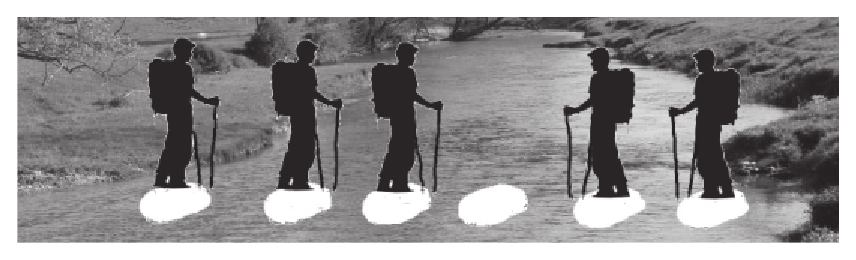
\includegraphics{randonneurs.eps}
  \end{center}


Le chemin de cailloux est défini par un tableau d'entiers :

\begin{center}
  \mintinline{OCaml}{type chemin_caillou = int array}
\end{center}

Dans ce tableau, un randonneur venant de la berge de gauche est représenté par un $1$, un randonneur issu de la berge de droite par un $2$, et un caillou libre par un $0$. Avec cette représentation, la figure ci-dessus correspond au tableau {\tt [|1; 1; 1; 0; 2; 2|]}. A partir de cette position, les mouvements possibles sont :
\begin{itemize}
    \item déplacement du premier randonneur de gauche : {\tt [|1; 1; 0; 1; 2; 2|]},
    \item saut du second randonneur de gauche par dessus le premier : {\tt [|1; 0; 1; 1; 2; 2|]}
    \item déplacement du premier randonneur de droite ; {\tt [|1; 1; 1; 2; 0; 2|]}
    \item saut du second randonneur de droite par dessus le premier : {\tt [|1; 1; 1; 2; 2; 0|]}
\end{itemize}
\quad

\Question{Écrire une fonction de signature \mintinline{Ocaml}{caillou_vide : chemin_caillou -> int} qui détermine la position du caillou inoccupé.}
\inputpartOCaml{traversee.ml}{}{}{3}{9}
\Question{
  Écrire une fonction de signature \mintinline{ocaml}{echange : chemin_caillou -> int -> int -> chemin_caillou} qui permute les valeurs codées sur deux cailloux et renvoie le tableau correspondant à la nouvelle position. Le tableau d'entiers initial représentant le chemin n'est pas modifié. On pourra utiliser ici la fonction \mintinline{ocaml}{copy} du module \mintinline{ocaml}{Array}.
}
\inputpartOCaml{traversee.ml}{}{}{11}{16}
\Question{  Écrire une fonction de signature \mintinline{ocaml}{randonneurG_avance : chemin_caillou -> bool} qui teste si, parmi les randonneurs venant de la berge de gauche, il en existe un qui puisse avancer (vers la droite).
}
\inputpartOCaml{traversee.ml}{}{}{18}{24}
\Question{
  Écrire une fonction de signature \mintinline{ocaml}{randonneurG_saute : chemin_caillou -> bool} qui teste si, parmi les randonneurs venant de la berge de gauche, il en existe un qui puisse sauter (vers la droite) au-dessus d'un randonneur.
}
\inputpartOCaml{traversee.ml}{}{}{34}{40}

  On supposera dans la suite les fonctions de signature \mintinline{ocaml}{randonneurD_avance : chemin_caillou -> bool} et \mintinline{ocaml}{randonneurD_saute : chemin_caillou -> bool} écrites de manière similaire pour les randonneurs venant de la berge de droite.

\Question{
  Écrire une fonction de signature \verb|mouvement_chemin : chemin_caillou -> chemin_caillou list| qui, en fonction de l'état du chemin, calcule la liste possible des états suivants après les opérations (si elles sont permises) :
  \begin{enumerate}
  \item[i)] déplacement d'un randonneur venant de la berge de gauche,
  \item[ii)] déplacement d'un randonneur venant de la berge de droite,
  \item[iii)] saut d'un randonneur venant de la berge de gauche,
  \item[iv)] saut d'un randonneur venant de la berge de droite.
  \end{enumerate}}
  \inputpartOCaml{traversee.ml}{}{}{50}{57}
\Question{Ecrire une fonction {\tt init\_chemin int -> int -> chemin\_caillou} qui prend en argument deux entiers {\tt ng} et {\tt nd} et renvoie le tableau correspondant à la  situation initiale de {\tt ng} randonneurs venant de la gauche et {\tt nd} randonneurs venant de la droite séparé par un caillou vide. Par exemple, {\tt init\_chemin 3 2} renvoie le tableau {\tt [| 1; 1; 1; 0; 2; 2 |]}.} 
\inputpartOCaml{traversee.ml}{}{}{72}{80}
\Question{
  Écrire une fonction de signature \verb|passage : int -> int -> chemin_caillou list|, utilisant la question précédente, telle que l'appel \verb|passage nG nD| résout le problème du passage de \verb|nG| randonneurs venant de la berge de gauche et \verb|nD| randonneurs venant de la berge de droite. Par exemple, \verb|passage 3 2| renvoie une liste d'états permettant de passer de {\tt [|1; 1; 1; 0; 2; 2|]} à {\tt [| 2; 2; 0; 1; 1; 1 |]}.
  % ERREUR SUJET :
  % j'ai fait une supposition sur le type attendu de la fonction qui ne pouvait pas être int -> int
}
\inputpartOCaml{traversee2.ml}{}{}{84}{96}

\end{Exercise}

\begin{Exercise}[title={Saut de valeur maximale}, origin={\bac {\sc capes nsi 2023}}]\\
Les fonctions demandées dans cet exercice sont à écrire en OCaml. \smallskip \\
Dans un tableau de flottants (type {\tt float} de OCaml) {\tt t} de taille {\tt n}, on appelle \textit{saut} un couple $(i,j)$ avec $0 \leq i \leq j <$ {\tt n  } et la \textit{valeur} d'un saut est la valeur {\tt t.(j)-t.(i)}. Le but de l'exercice est de rechercher un saut de valeur maximale dans un tableau. Par exemple, dans le tableau {\tt [| 2.0; 0.2; 3.0; 5.3; 2.0 |]}, un tel saut est {\tt (1, 3)} (car {\tt 0.2} et {\tt 5.3} sont aux indices 1 et 3 respectivement) et la valeur maximale d'un saut est donc {\tt 5.3 - 0.2 = 5.1}.

\Question{Ecrire une fonction {\tt valeur float array -> int -> int -> float} qui prend en argument un tableau ainsi que deux indices {\tt i} et {\tt j} et renvoie la valeur du saut {\tt (i,j)}. Par exemple  sur le tableau {\tt [|2.0; 0.2; 3.0; 5.3; 2.0|]} avec les indices 0 et 2 cette fonction renvoie {\tt 1.0} (car {\tt t.(2)-t.(0) = 1.0}).} 
\inputpartOCaml{sautmax.ml}{}{}{2}{2}
\Question{Donner un exemple de tableau avec exactement deux sauts de valeur maximale et préciser ces sauts.}
\tcor{La liste {\tt [2, 6, 1, 5]} possède deux sauts de valeurs maximale : {\tt (0,1)} et {\tt (2,3)} (ces deux sauts ont une valeur de 4)} 
\Question{À l'aide d'un contre-exemple, montrer qu'on ne peut pas se contenter de chercher le minimum et le maximum d'un tableau pour trouver un saut de valeur maximale.}
\tcor{Dans la liste {\tt [2, 6, 1, 5]} le minimum est à l'indice 2 (c'est 1) et le maximum à l'indice 1 (c'est 3) et comme le minimum est après le maximum ce n'est pas le saut maximal.} 
\Question{Écrire une fonction {\tt saut\_max\_naif} qui renvoie un saut de valeur maximale dans un tableau de taille {\tt n} en testant tous les couples $(i,j)$ tels que $0 \leq i \leq j <$ {\tt n}.\label{naif}}\medskip
\inputpartOCaml{sautmax.ml}{}{}{4}{12}

On propose maintenant d'utiliser une méthode diviser pour régner afin de calculer la valeur maximale d'un saut. On note $n$ la taille du tableau {\tt t} et $p = \lfloor \frac{n}{2} \rfloor$ (où $\lfloor \; \rfloor$ désigne la partie entière). On souhaite calculer :
\begin{itemize}
    \item $(i_g,j_g)$ un saut de valeur maximale lorsque $j_g < p$
    \item $(i_d,j_d)$ un saut de valeur maximale lorsque $id \geqslant p$
    \item $(i_m,j_m)$ un saut de valeur maximal lorsque $i_m < p < j_m$
\end{itemize}

\Question{Justifier qu'un saut de valeur maximale du tableau {\tt t} est nécessairement un des trois ci-dessus.}
\tcor{Un saut de valeur maximal $(i,j)$ du tableau {\tt t} est tel que $i \leqslant j$ et donc on est forcément dans l'une des trois situations suivantes :
\begin{itemize}
  \item $i\leqslant j<p$ et donc c'est un saut de valeur maximale du sous tableau constitué des éléments d'indice $0\dots p-1$
  \item $p \leqslant i \leqslant j$ et donc c'est un saut de valeur maximale du sous tableau constitué des éléments d'indice $p\dots n-1$
  \item $i < p < j$
\end{itemize}  
Ce qui correspond bien aux trois situations décrites ci-dessus.
}
\Question{Justifier que $i_m$ est nécessairement l'indice d'une valeur minimale dans la moitié gauche de {\tt t} (on admettra que de même $j_m$ est nécessairement l'indice d'une valeur maximale dans la moitié droite de {\tt t}).}
\tcor{On raisonne par l'absurde, si tel n'était pas le cas, on aurait une valeur d'indice $q$ dans la moitié gauche strictement inférieur à $t[i_m]$ et donc le saut $(q,j_m)$ aurait une valeur supérieure au saut $(i_m,j_m)$ ce qui contredit que $(i_m,j_m)$ est un saut de valeur maximale.}
\Question{Ecrire une fonction {\tt saut\_max\_aux} qui prend en argument un tableau {\tt} ainsi que deux entiers {\tt a} et {\tt b} (avec {\tt a<b}) et renvoie un quadruplet constitué des deux indices d'un saut de valeur maximale dans {\tt t} entre les deux indices {\tt a} (inclus) et {\tt b} (exclu) ainsi que les indices d'un minimum et d'un maximum de {\tt t} entre ces deux mêmes indices. Par exemple {\tt saut\_max\_aux [| 2.0; 5.0; 3.0; 4.0; 6.0; 1.0|] 2 6} doit renvoyer {\tt (2, 4, 5, 4)} car entre les indices 2 (inclus) et 6 (exclu), le saut de valeur maximale est {\tt (2,4)} (de valeur {\tt 3.0}), le minimum est {\tt 1} et le maximum est {\tt 6}.\\
\textit{Cette fonction doit être récursive et utiliser la méthode diviser pour régner}.
}
\inputpartOCaml{sautmax.ml}{}{}{14}{27}
\Question{En déduire une fonction de {\tt saut\_max\_dpr} qui renvoie un saut de valeur maximale du tableau donné en argument.}
\inputpartOCaml{sautmax.ml}{}{}{29}{31}

\Question{Donner (en les justifiant) les complexités des deux méthodes (naïves et diviser pour régner).}
\tcor{
  La méthode naïve a une complexité quadratique car on a deux boucles de taille $n$ imbriquées
}
\end{Exercise}

\end{document}